\chapter{继承}

在本章中我们将设计一个来玩扑克的类。如果你不玩扑克,你可以在\url{wikipedia.org/wiki/Poker}中阅读相关信息,但你不必这么做,做练习时我会告诉你一些所需要的信息。

\index{玩扑克,Anglo-American}
\index{纸牌,玩}
\index{扑克}

如果你不熟悉如何玩扑克,你可以阅读\url{wikipedia.org/wiki/Playing_cards}中的内容。


\section{扑克对象}

一副牌有52张牌,每一张属于4个花色和13个等级。4中花色是黑桃、红桃、草花和方块。13个等级是Ace,2,3,4,5,6,7,8,9,10,J,Q和K。对于不同的游戏,Ace肯能比2大,也可能比2小。

\index{等级}
\index{花色}

如果我们要定义一个纸牌的对象,显然其属性有{\tt 等级}和{\tt 花色},但是属性的数据类型应该如何选择?一个方法是使用字符串,如用\verb"'Spade'"描述花色, \verb"'Queen'"描述等级。这么做的一个问题在于实现花色或等级的比较不是很容易。

\index{编码}
\index{加密}
\index{映射}
\index{表示}

另一个方法是使用整数对等级和花色{\bf 编码}。在这里,“编码”指我们将定义一个数字和花色以及数字和等级之间的映射。这种映射不是秘密的(区别“加密”)。

例如,下面的表格给出了花色和对应整数编码:

\beforefig
\begin{tabular}{l c l}
Spades & $\mapsto$ & 3 \\
Hearts & $\mapsto$ & 2 \\
Diamonds & $\mapsto$ & 1 \\
Clubs & $\mapsto$ & 0
\end{tabular}
\afterfig

这个编码简化了卡片的比较,由于高的花色映射为大的数,我们可以通过比较编码来比较花色。

等级的映射相对更明显,每个数字等级映射为对应的整数,对于其他卡片:

\beforefig
\begin{tabular}{l c l}
Jack & $\mapsto$ & 11 \\
Queen & $\mapsto$ & 12 \\
King & $\mapsto$ & 13 \\
\end{tabular}
\afterfig

我使用$\mapsto$符号来突出这些映射不是Python程序实现的。它们属于程序的设计,但它们不直接的表现在代码中。

\index{Card类}
\index{类!Card}

{\tt Card}类的定义如下:

\beforeverb
\begin{verbatim}
class Card(object):
    """represents a standard playing card."""

    def __init__(self, suit=0, rank=2):
        self.suit = suit
        self.rank = rank
\end{verbatim}
\afterverb
%
Init方法有两个可选参数,默认的卡片是草花2。

\index{init方法}
\index{方法!init}

如果要创建一个卡片,你可以调用{\tt Card},并传入你要的花色和等级。

\beforeverb
\begin{verbatim}
queen_of_diamonds = Card(1, 12)
\end{verbatim}
\afterverb
%


\section{类属性}

\index{类属性}
\index{属性!类}

为了以适合人类阅读的格式打印卡片对象,我们需要整数代码到对应花色和等级的映射。一个自然的方法是使用字符串列表,我们将这两个列表赋值给{\bf 类属性}:

\beforeverb
\begin{verbatim}
# inside class Card:

    suit_names = ['Clubs', 'Diamonds', 'Hearts', 'Spades']
    rank_names = [None, 'Ace', '2', '3', '4', '5', '6', '7', 
              '8', '9', '10', 'Jack', 'Queen', 'King']

    def __str__(self):
        return '%s of %s' % (Card.rank_names[self.rank],
                             Card.suit_names[self.suit])
\end{verbatim}
\afterverb
%
定义在类内部任何函数外的变量,如\verb"suit_names"和\verb"rank_names",被称为类属性,因为它们和类对象{\tt Card}像关联。

\index{实例属性}
\index{属性!实例}

该术语区别类似{\tt suit}和{\tt rank}的变量,它们被称为{\bf 实例属性},因为它们和一个特定的实例相关联。

\index{点符号}

两种属性都通过点符号访问。例如,在\verb"__str__"里,{\tt self}是一个卡片对象,{\tt self.rank}是它的等级。类似的,{\tt Card}是一个类对象,\verb"Card.rank_names"是一个和类关联的字符串列表。

每个卡片都有自己的{\tt 花色}和{\tt 等级},但是有一个\verb"suit_names"和\verb"rank_names"的备份。

将这些结合起来,表达式\verb"Card.rank_names[self.rank]"意思是“从{\tt self}对象中使用属性{\tt rank}作为下标,访问{\tt Card}类中的\verb"rank_names"列表,选择对应的字符串”。

\verb"rank_names"中的第一个元素是{\tt None},因为没有等级为零的卡片。通过引入{\tt None}作为占位符,我们很好的将下标2映射为字符串\verb"'2'",以此类推。若不使用这种方法,我们可以使用一个字典,而不是一个列表。

基于我们已有的方法,我们可以创建并打印卡片:

\beforeverb
\begin{verbatim}
>>> card1 = Card(2, 11)
>>> print card1
Jack of Hearts
\end{verbatim}
\afterverb
%
下面给出{\tt Card}类对象和一个卡片实例的图:

\index{状态图}
\index{图!状态}
\index{对象图}
\index{图!对象}

\beforefig
\centerline{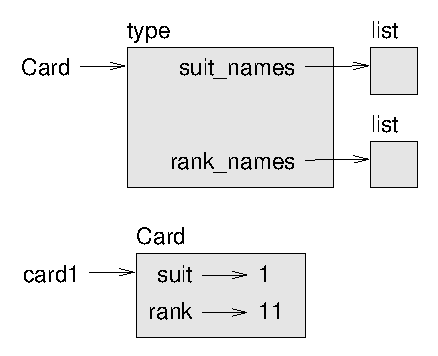
\includegraphics{figs/card1.eps}}
\afterfig

{\tt Card}是一个类对象,它的数据类型为{\tt type}。{\tt card1}的类型为{\tt Card}。(为了节省空间,我没有画出\verb"suit_names"和\verb"rank_names"的内容)。


\section{比较卡片}
\label{比较卡片}

\index{运算夫!关系}
\index{关系运算夫}

对于内建类型,关系运算符(如{\tt <},{\tt >},{\tt ==}等)可以比较它们的值。对于用户定义的类型,我们可以通过提供\verb"__cmp__"函数来重载内建运算符的行为。


\verb"__cmp__"接受两个参数,{\tt self}和{\tt other},如果第一个对象大则返回一个正数,如果第一个对象小则返回一个负数,如果两者两等则返回0。

\index{重载}
\index{运算符重载}

卡片的正确顺序不是很明显。例如一个草花3和一个方块2哪个大?一个等级更高,而另一个花色更高。为了比较卡片,你需要确定等级和花色哪个更重要。

答案取决于你玩的是什么游戏。为了简单起见,我们任意的选择花色更为重要,因此所有的黑桃都大于任意方块,依此类推。

\index{cmp 方法@\_\_cmp\_\_ 方法}
\index{方法!\_\_cmp\_\_}

当这个决定后,我们可以编写\verb"__cmp__":

\beforeverb
\begin{verbatim}
# inside class Card:

    def __cmp__(self, other):
        # check the suits
        if self.suit > other.suit: return 1
        if self.suit < other.suit: return -1

        # suits are the same... check ranks
        if self.rank > other.rank: return 1
        if self.rank < other.rank: return -1

        # ranks are the same... it's a tie
        return 0    
\end{verbatim}
\afterverb
%
你可以使用元组比较编写更简洁的程序:

\index{元组!比较}
\index{比较!元组}

\beforeverb
\begin{verbatim}
# inside class Card:

    def __cmp__(self, other):
        t1 = self.suit, self.rank
        t2 = other.suit, other.rank
        return cmp(t1, t2)
\end{verbatim}
\afterverb
%
内建函数{\tt cmp}和方法\verb"__cmp__"有相同的接口:它读取两个值,如果第一个更大则返回一个正数,第二个更大则返回一个负数,如果相等则返回0。

\index{cmp函数}
\index{函数!cmp}


\begin{ex}
为时间对象编写方法\verb"__cmp__"。提示:你可以使用元组比较,也可以考虑使用整数减法。

%    def __cmp__(self, other):
%        return time_to_int(self) - time_to_int(other)

%If {\tt self} is later than {\tt other}, the result is
%a positive number.  If {\tt other} is later, the result
%is negative.  And if {\tt self} and {\tt other} are equal
%(but not necessarily identical)
%the result is zero.

\end{ex}


\section{纸牌}
\index{列表!对象的}
\index{纸牌,玩卡片}

现在我们有卡片对象,下一步是定义纸牌。由于纸牌是由卡片组成的,自然的想法是每个纸牌将一个卡片的列表作为它的属性。

\index{init方法}
\index{方法!init}

下面是{\tt 纸牌}的类定义。初始化方法创建{\tt 卡片}属性,并生成标准的52张卡片:

\index{组成}
\index{循环!嵌套}

\index{纸牌类}
\index{类!纸牌}

\beforeverb
\begin{verbatim}
class Deck(object):

    def __init__(self):
        self.cards = []
        for suit in range(4):
            for rank in range(1, 14):
                card = Card(suit, rank)
                self.cards.append(card)
\end{verbatim}
\afterverb
%
生成纸牌最简单的方法是使用一个嵌套的循环。外层循环枚举0到3的花色,内层循环枚举1到13的等级。每次迭代创建一个对应当前花色和等级的新卡片,并附加在{\tt self.cards}后。

\index{append方法}
\index{方法!append}


\section{打印纸牌}
\label{打印纸牌}

\index{str 方法@\_\_str\_\_ 方法}
\index{方法!\_\_str\_\_}

下面是{\tt 纸牌}的\verb"__str__"方法:

\beforeverb
\begin{verbatim}
#inside class Deck:

    def __str__(self):
        res = []
        for card in self.cards:
            res.append(str(card))
        return '\n'.join(res)
\end{verbatim}
\afterverb
%
这个方法演示了汇聚大字符串的有效的方法:建立一个字符串列表,然后使用{\tt join}方法。内建函数{\tt str}对每个卡片调用\verb"__str__"方法,并返回表征的字符串。

\index{汇聚!字符串}
\index{字符串!汇聚}
\index{join方法}
\index{方法!join}
\index{新行}

由于我们在新行符号上调用{\tt join},卡片通过新行符分割。下面是结果:

\beforeverb
\begin{verbatim}
>>> deck = Deck()
>>> print deck
Ace of Clubs
2 of Clubs
3 of Clubs
...
10 of Spades
Jack of Spades
Queen of Spades
King of Spades
\end{verbatim}
\afterverb
%
虽然结果看起来是52行,实际上它是一个包含换行符的一个长字符串。


\section{添加,删除,洗牌,理牌}

对于卡片,我们需要一个从纸牌中删除一张卡片并返回改纸牌的方法。列表的{\tt pop}方法提供了一个便捷的实现方式:

\index{pop方法}
\index{方法!pop}

\beforeverb
\begin{verbatim}
#inside class Deck:

    def pop_card(self):
        return self.cards.pop()
\end{verbatim}
\afterverb
%
由于{\tt pop}删除列表中{\em 最后}一张卡片,我们是纸牌底部进行操作。在现实生活中从底部操作是不可取的\footnote{参考\url{wikipedia.org/wiki/Bottom_dealing}},但在这里也是行得通的。

\index{append方法}
\index{方法!append}

为了添加一张卡片,我们可以使用列表的{\tt append}方法:

\beforeverb
\begin{verbatim}
#inside class Deck:

    def add_card(self, card):
        self.cards.append(card)
\end{verbatim}
\afterverb
%
类似这种调用其他函数,本身不做很多具体工作的方法有时被称为{\bf 饰面}。这个词来自木工行业,通常人们将一片很薄的好木材黏贴在一块便宜的木材的表面。

\index{饰面}

在本例中我们定义个一个“单薄”的方法,使列表的操作适用于纸牌。

作为另一个例子,我们可以编写纸牌方法{\tt shuffle},调用{\tt random}模块中的{\tt shuffle}函数: 

\index{random模块}
\index{模块!random}
\index{shuffle函数}
\index{函数!shuffle}

\beforeverb
\begin{verbatim}
# inside class Deck:
            
    def shuffle(self):
        random.shuffle(self.cards)
\end{verbatim}
\afterverb
%
不要忘了导入{\tt random}模块。

\begin{ex}
\index{sort方法}
\index{方法!sort}

编写纸牌方法{\tt sort},通过调用列表方法{\tt sort}对{\tt 纸牌}中的卡片进行排序。{\tt sort}适用我们定义的\verb"__cmp__"方法来决定排序顺序。
\end{ex}



\section{继成}

\index{继成}
\index{面向对象编程}

和面向对象编程最相关的语言特点是{\bf 继成}。继成是通过修改已有的类来创建新的类的能力。

\index{父类}
\index{子类}
\index{类!子}
\index{子类}
\index{超类}

之所以称为“继成”是因为新的类继成了已有类的方法。换言之,已有类被称为{\bf 父类},新创建的类被称为{\bf 子类}。

例如,我们要创建一个类来表示“手牌”,即一个玩家手中持有的牌。手牌类似纸牌:它们都是卡片的集合,都需要类似添加和删除卡片的操作。

手牌同时区别于纸牌:我们需要手牌有一些操作,但这些操作对纸牌来说没有意义。例如,在扑克中我们需要比较两个手牌来决定谁获胜。在桥牌中,我们需要计算手牌的分数,以便要价。

两个类的相似关系和不同点导致了它们的继成关系。

子类的定义和其他类定义相同,但父类的名字出现在括号中:

\index{括号!父类在}
\index{父类}
\index{类!父}
\index{Hand类}
\index{类!Hand}

\beforeverb
\begin{verbatim}
class Hand(Deck):
    """represents a hand of playing cards"""
\end{verbatim}
\afterverb
%
该定义表示{\tt Hand}继成{\tt Deck},这意味着我们可以想纸牌一样对手牌使用类似\verb"pop_card"和\verb"add_card"的方法。

{\tt Hand}同时继成了{\tt Deck}的\verb"__init__",但这并不是我们想要的:手牌的{\tt cards}属性应该被初始化为一个空的列表,而不是塞满52张新牌。


\index{重载}
\index{init方法}
\index{方法!init}

如果我们给{\tt Hand}提供一个初始化方法,它将重载{\tt Deck}中的方法:

\beforeverb
\begin{verbatim}
# inside class Hand:

    def __init__(self, label=''):
        self.cards = []
        self.label = label
\end{verbatim}
\afterverb
%
因此当你创建了一个手牌对象,Python调用这个初始化方法:

\beforeverb
\begin{verbatim}
>>> hand = Hand('new hand')
>>> print hand.cards
[]
>>> print hand.label
new hand
\end{verbatim}
\afterverb
%
但是其他方法从{\tt Deck}继成,所以我们可以使用\verb"pop_card"和\verb"add_card"来处理卡片:

\beforeverb
\begin{verbatim}
>>> deck = Deck()
>>> card = deck.pop_card()
>>> hand.add_card(card)
>>> print hand
King of Spades
\end{verbatim}
\afterverb
%
自然的下一步是将这些代码封装成\verb"move_cards"方法:

\index{封装}

\beforeverb
\begin{verbatim}
#inside class Deck:

    def move_cards(self, hand, num):
        for i in range(num):
            hand.add_card(self.pop_card())
\end{verbatim}
\afterverb
%
\verb"move_cards"读取两个参数,一个为手牌对象,一个为要处理的卡片数。它同时修改{\tt self}和{\tt hand},并返回{\tt None}。

在有的游戏中,卡片在不同手牌中移动,或者从手牌移动到台面牌。你可以使用\verb"move_cards"来进行任何这些操作:{\tt self}可以是手牌或者桌面牌,{\tt hand}同样可以是{\tt 桌面牌},虽然它名字叫手牌。

\begin{ex}
编写纸牌方法\verb"deal_hands",读取两个参数,分别是手牌的个数和每个手牌的卡片个数,并根据这个数字创建手牌对象,返回一个手牌对象列表。
\end{ex}
继成是一个有用的特性。通过使用继成可以将一些重复行的程序写得更优雅。继成使得代码重用更容易,你可以自定义父类的行为,而不需要去改变它。在某些情况下,继成结构反应了现实中问题的结构,使得问题容易理解。

另一方面,继成会使得程序难以阅读。当一个方法被调用时,有时方法的定义的位置不是很清楚。相关的代码可能散布在多个模块中。同时,很多可以用继成做的事情同样可以不用继成来实现,甚至做得更好。


\section{类图}

目前位置我们见过了栈图,它现实了程序的状态,对象图,它现实了对象的属性和值。这些图是程序执行过程中的快照,因此它们随程序的执行而改变。

同时它们非常详细,有时对某些应用太详细了。类图是个相对抽象的表示程序结构的图,它显示了类的结构和类之间的关系,而不是显示每一个对象。

存在以下几种类的关系:

\begin{itemize}

\item 类中的一个对象包含另一个类的对象的引用。例如,每个长方形包含一个点的应用,每个纸牌包含多个卡片的引用。这类关系被称为{\bf 包含},正如“长方形包含一个点”。

\item 一个类是另一个类的继成。这种关系被称为{\bf 是},正如“手牌是纸牌的一种”。

\item 一个类也许决定于另一个类,即一个类的改动要求其他类的改动。

\end{itemize}

\index{属于关系}
\index{包含关系}
\index{类图}
\index{图!类}
\index{UML}

{\bf 类图}是图形化的表示这些关系的图\footnote{我在这里使用的图类似UML(参考\url{wikipedia.org/wiki/Unified_Modeling_Language})}。例如,下面的图显示了{\tt Card},{\tt Deck}和{\tt Hand}的关系。

\beforefig
\centerline{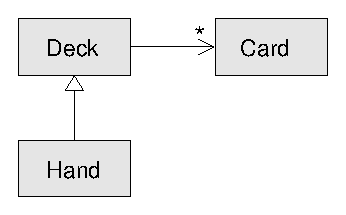
\includegraphics{figs/class1.eps}}
\afterfig

空心三角箭头表示“属于关系”,在本例中表示手牌继成了纸牌。

标准箭头表示“有关系”,在本例中纸牌有卡片的引用。

\index{多态(在类图中)}

在箭头头部的新号({\tt *})表示{\bf 多态}。它指示了纸牌中有多少张卡片。多态可以是一个简单的数字,如{\tt 52},一个范围,如{\tt 5..7},或一个新号,表示纸牌可以有任何多的卡片。

更详细的图将显示纸牌事实上又一个卡片{\em 列表},但是通常类似列表和字典的内建类型不出现在类图中。

\begin{ex}
阅读{\tt TurtleWorld.py},{\tt World.py}和{\tt Gui.py},绘制类图来显示它们之间的关系。
\end{ex}


\section{调试}
\index{调试}

继承使得调试成为一个挑战,因为当你对一个对象调用方法是,你也许不知道哪个方法被调用。

\index{多态}

假设你编写了一个手牌对象的函数,你希望它能适用于任何手牌,如扑克手牌,桥牌手牌等。假设你调用了类似{\tt shuffle}的方法,你也许调用的是定义在{\tt 纸牌}中的方法,但是如果某个子类重载了这个方法,你会得到那个版本的方法。

\index{执行流程}
当你不确定程序执行的流程,最简单的方法是在相关的方法的开始部分添加打印语句。如果{\tt Deck.shuffle}打印类似{\tt Running Deck.shuffle}的语句,那么当程序执行时它将追踪执行的流程。

另一个方法是使用下面的函数,它接受一个对象和一个方法名(以字符串的形式),返回提供该方法定义的类:

\beforeverb
\begin{verbatim}
def find_defining_class(obj, meth_name):
    for ty in type(obj).mro():
        if meth_name in ty.__dict__:
            return ty
\end{verbatim}
\afterverb
%
下面给出一个例子:

\beforeverb
\begin{verbatim}
>>> hand = Hand()
>>> print find_defining_class(hand, 'shuffle')
<class 'Card.Deck'>
\end{verbatim}
\afterverb
%
因此这个手牌的{\tt shuffle}方法来自{\tt 纸牌}。

\index{mro方法}
\index{方法!mro}
\index{方法解析顺序}

\verb"find_defining_class"使用{\tt mro}方法得到用于查找方法的类对象(类型)列表。“MRO”指“method resolution order”,即方法解析顺序。

\index{重载}
\index{接口}
\index{先决条件}
\index{后决条件}

以下是程序设计的建议:每当你重载一个方法,新方法的接口应该和原方法相同。它们应使用相同的参数,返回相同的类型,符合相同的先决条件和后决条件。如果你遵守这些规则,你会发现任何使用于超类实例(如纸牌)的函数同样使用于子类实例(如手牌或扑克手牌)。

如果你违反了这些规则,你的代码很肯会崩溃。


\section{术语}

\begin{description}

\item[编码:] 通过建立映射使用一个集合的值表示另一个集合的值。
\index{编码}

\item[类属性:] 和类对象关联的属性。类属性定义在类定义内部,方法定义外部。
\index{类属性}
\index{属性!类}

\item[实例属性:] 和类的实例相关的属性。
\index{实例属性}
\index{属性!实例}

\item[饰面:] 为另一个函数提供不同的接口而不进行许多计算的方法或函数。
\index{饰面}

\item[继承:] 通过修改先前定义的类来创建新的类的能力。
\index{继承}

\item[父类:] 被子类继承的类。
\index{父类}

\item[子类:] 通过继承已有的类而创建的新的类。
\index{子类}
\index{类!子}

\item[属于关系:] 子类和父类之间的关系。
\index{属于关系}

\item[包含关系:] 两个类之间的关系,其中的一个类包含另一个类的引用。
\index{包含关系}

\item[类图:] 表示程序中的类以及类之间的关系的图。
\index{类图}
\index{图!类}

\item[多态:] 类图中的标记,对于包含关系,该标记说明了对其他类的引用的数量。
\index{多态(在类图中)}

\end{description}


\section{练习}

\begin{ex}
\index{扑克}

下面是扑克中肯能的手牌,以大小升序排列(概率降序):

\begin{description}

\item[对子:] 等级相同的两张牌。
\vspace{-0.05in}

\item[双对:] 等级相同的两对对子。
\vspace{-0.05in}

\item[相同的3个:] 等级相同的3张卡片。
\vspace{-0.05in}

\item[顺子:] 5张等级连续的卡片(aces可以为高或低,因此{\tt Ace-2-3-4-5}是个顺子,{\tt 10-Jack-Queen-King-Ace}也是顺子,但是{\tt Queen-King-Ace-2-3}不是)。
\vspace{-0.05in}

\item[同花:] 5张花色相同的卡片。
\vspace{-0.05in}

\item[3张相同和2张相同的牌:] 3张牌等级相同,另2张牌等级相同。
\vspace{-0.05in}

\item[相同的4个] 等级相同的4张牌。
\vspace{-0.05in}

\item[同花顺:] 5张花色相同的顺子。
\vspace{-0.05in}

\end{description}
%
本练习的目的是估计抽到不同的手牌的概率。

\begin{enumerate}

\item 从\url{thinkpython.com/code}下载下列文件:

\begin{description}

\item[{\tt Card.py}]: 本章中{\tt Card},{\tt Deck}和{\tt Hand}的完整版本。

\item[{\tt PokerHand.py}]: 未完成的手牌的类,包含一些测试代码。

\end{description}
%
\item 如果你运行{\tt PokerHand.py},它将抽取7张手牌,并检查是否包含同花顺。在你继续前请仔细阅读代码。

\item 在{\tt PokerHand.py}添加方法\verb"has_pair",\verb"has_twopair"等,根据相关准则进行判断并返回True或者False。你的代码应使用于任意张数的手牌(虽然5和7是最常见的数量)。

\item 编写方法{\tt classify},找出手牌中值最大的分类,并记录在{\tt label}属性中。例如,一个7张的手牌可能有一个顺子和一对,那么应该标记为“顺子”。

\item 当你确信你的分类方法工作正常,下一步是估计不同手牌出现的概率。在{\tt PokerHand.py}中编写函数,对一副牌进行洗牌,然后分为若干手牌,对手牌分类,统计不同分类出现的次数。

\item 打印分类和概率的表。多次运行程序,直到输出稳定到一个合理的精度。将你的结果和\url{wikipedia.org/wiki/Hand_rankings}比较。

\end{enumerate}
\end{ex}


\begin{ex}

\index{沼泽}
\index{TurtleWorld}
本练习使用章节~\ref{turtlechap}的TurtleWorld。
你将编写代码,让乌龟玩贴标签的游戏。如果你不熟悉游戏规则,参考\url{wikipedia.org/wiki/Tag_(game)}。

\begin{enumerate}

\item 下载\url{thinkpython.com/code/Wobbler.py}并运行。你将看到乌龟世界里有3只乌龟。如果你按下{\sf Run}按钮,乌龟将随机移动。

\item 阅读代码,了解它是如何工作的。{\tt 闲逛者}类继承{\tt 乌龟}类,这意味着{\tt 乌龟}的方法{\tt lt},{\tt rt},{\tt fd}和{\tt bk}同样适用于闲逛者。

{\tt step}方法由乌龟世界调用。它调用{\tt steer},令乌龟朝向指定的方向。{\tt wobble}根据乌龟的笨拙程度随机的转向,{\tt move}根据乌龟的速度向前移动一定的距离。

\index{跟踪者}

\item 创建{\tt Tagger.py},导入{\tt Wobbler},定义类{\tt Tagger},继承{\tt Wobbler}。以{\tt Tagger}的类对象作为参数的调用\verb"make_world"。

\item 在{\tt Tagger}中添加{\tt steer}方法,重载{\tt Wobbler}中的函数。作为起步练习,编写始终将乌龟指向原点的版本。提示:使用数学函数{\tt atan2}和乌龟属性{\tt x},{\tt y}和{\tt heading}。

\item 修改{\tt steer},将乌龟约束在边界内。为了调试,你可以使用{\sf Step}按钮,它将对每个乌龟调用{\tt step}。

\item 修改{\tt steer},令每只乌龟朝向离它最近的邻居。提示:乌龟有属性{\tt world},是它们所在的乌龟世界的引用,而乌龟世界有属性{\tt animals},对应所有乌龟的列表。

\item 修改{\tt steer}让乌龟玩贴标签游戏。你可以在{\tt Tagger}上添加方法,并重载{\tt steer}和\verb"__init__",但你不能修改或重载{\tt step},{\tt wobble}或{\tt move}。另外{\tt steer}允许改变乌龟的方向,但不能改变位置。

修改规则和你的{\tt steer}方法,增加游戏的质量。例如,慢的乌龟应该有机会给快的乌龟贴上标签。

\end{enumerate}

你可以在\url{thinkpython.com/code/Tagger.py}下载到我的程序。
\end{ex}


